\documentclass[12pt,letterpaper]{article}
\usepackage{graphicx}
\usepackage{fullpage}
\usepackage{color}
\usepackage{listings}

\lstset{
  language=Python,
	basicstyle=\small\ttfamily,
	keywordstyle=\color{blue},
	commentstyle=\color{green}\emph,
	stringstyle=\color{red},
	showstringspaces=false,
	breaklines=true}
	
\lstset{
	morekeywords={open,write,close,append,int,float,dict,dot},
	morekeywords={defaultdict,list,math,re,shape,dtype,range,sorted,len,join,map,str}
	}
	
\begin{document}

\textwidth 6.5in
\baselineskip 18pt

\title{Optimization technique to generate MODFLOW RIV and SFR datasets from NHDPlus}
\author{Howard  Reeves, Mike Fienen, Andrew Leaf, and Daniel Feinstein}
\date{\today}

\maketitle

\section{Introduction}
MODFLOW models that include groundwater/surface-water interaction as a major component of
the analysis benefit from the streamflow routing (SFR) package compared to the more traditional
river (RIV) package because SFR allows stream stage to vary and does not provide an infinite supply
of water to the groundwater system.  Estimation of stream stage through SFR provides improved estimates of
streamflow capture by wells, and capture will be of particular interest for the glacial aquifer
study.  

The SFR package requires more input data than RIV, in particular the streambed elevations assigned
to MODFLOW cells must be routed: the elevation of the streambed in upstream cells must be greater than, 
or at a minimum equal to, the streambed elevation of the next downstream cell.  This prevents backwater
effects in SFR that can disrupt the estimated stage and lead to errors in the simulation.  Note that,
while not technically required, the RIV package benefits from a routed network.  If the stream network is
not routed within implementation of a RIV package, internal circulation of groundwater from RIV cells with higher elevation to adjacent RIV cells with lower elevation confounds the groundwater budget by overestimating
losing and gaining cells.  A routed stream network, therefore, is a major requirement for regional 
groundwater availability models.  Creation of a routed stream network, however, can be a major expense
of model development and one of its most labor-intensive tasks.

The NHDPlus dataset has both routing and elevation information, and it may
provide the data needed for regional groundwater-flow models. Python scripts have been written to do
much of the processing necessary to build a routed RIV or SFR package given the NHDPlus
data and a MODFLOW grid.  The scripts currently identify stream segments that have errors
in the underlying data caused by problems in the NHDPlus or in the intersection of the NHDPlus
with the grid (for example, a stream near the boundary of the grid may leave and re-enter the
grid presenting challenges to the routing).  The scripts, however, are still fairly {\em ad hoc} and
would benefit from more development and from an interface that would help the user through
the process.  In addition, we have identified the need to optimize the final streambed elevations and
have identified potential techniques that can be applied to this optimization.

\section{Problem statement}
Write a set of python scripts and an interface that will work with ArcGIS to facilitate the use of NHDPlus to generate a routed stream network for an arbitrary MODFLOW grid and build RIV or SFR datasets.  


\section{Overview of existing scripts and approach to build stream network from NHDPlus}
The existing scripts use the python module arcpy and the ArcToolbox for Arc 10.  In the current
form, the user must do some GIS processing to prepare to use the scripts. First, a MODFLOW grid
is prepared and exported as a shapefile with a known projection. The NHDPlus (version 2)
datafile for flowlines is then projected to match the target MODFLOW grid
and clipped to the MODFLOW grid.  GIS commands are used to intersect the flowlines and 
grid shapefile to yield a shapefile with separate pieces of the flowline for each 
grid cell. Additional work is required for the current scripts to allow
for the stream network to intersect multiple layers. After these steps, 
the intersected parts of the stream segment become reaches for SFR, and the stream arc designed by a single
COMID in NHDPlus becomes the SFR segment.  One advantage of using NHDPlus in this way is 
COMID in NHD/NHDPlus also may be identified using its reach number and events may be
indexed to the dataset by a reach number and distance along the reach.  Streamgages and
other events that have already been added to the NHD/NHDPlus datasets can be easily
related to the MODFLOW grid.

\begin{figure}[ht]
	\centering		  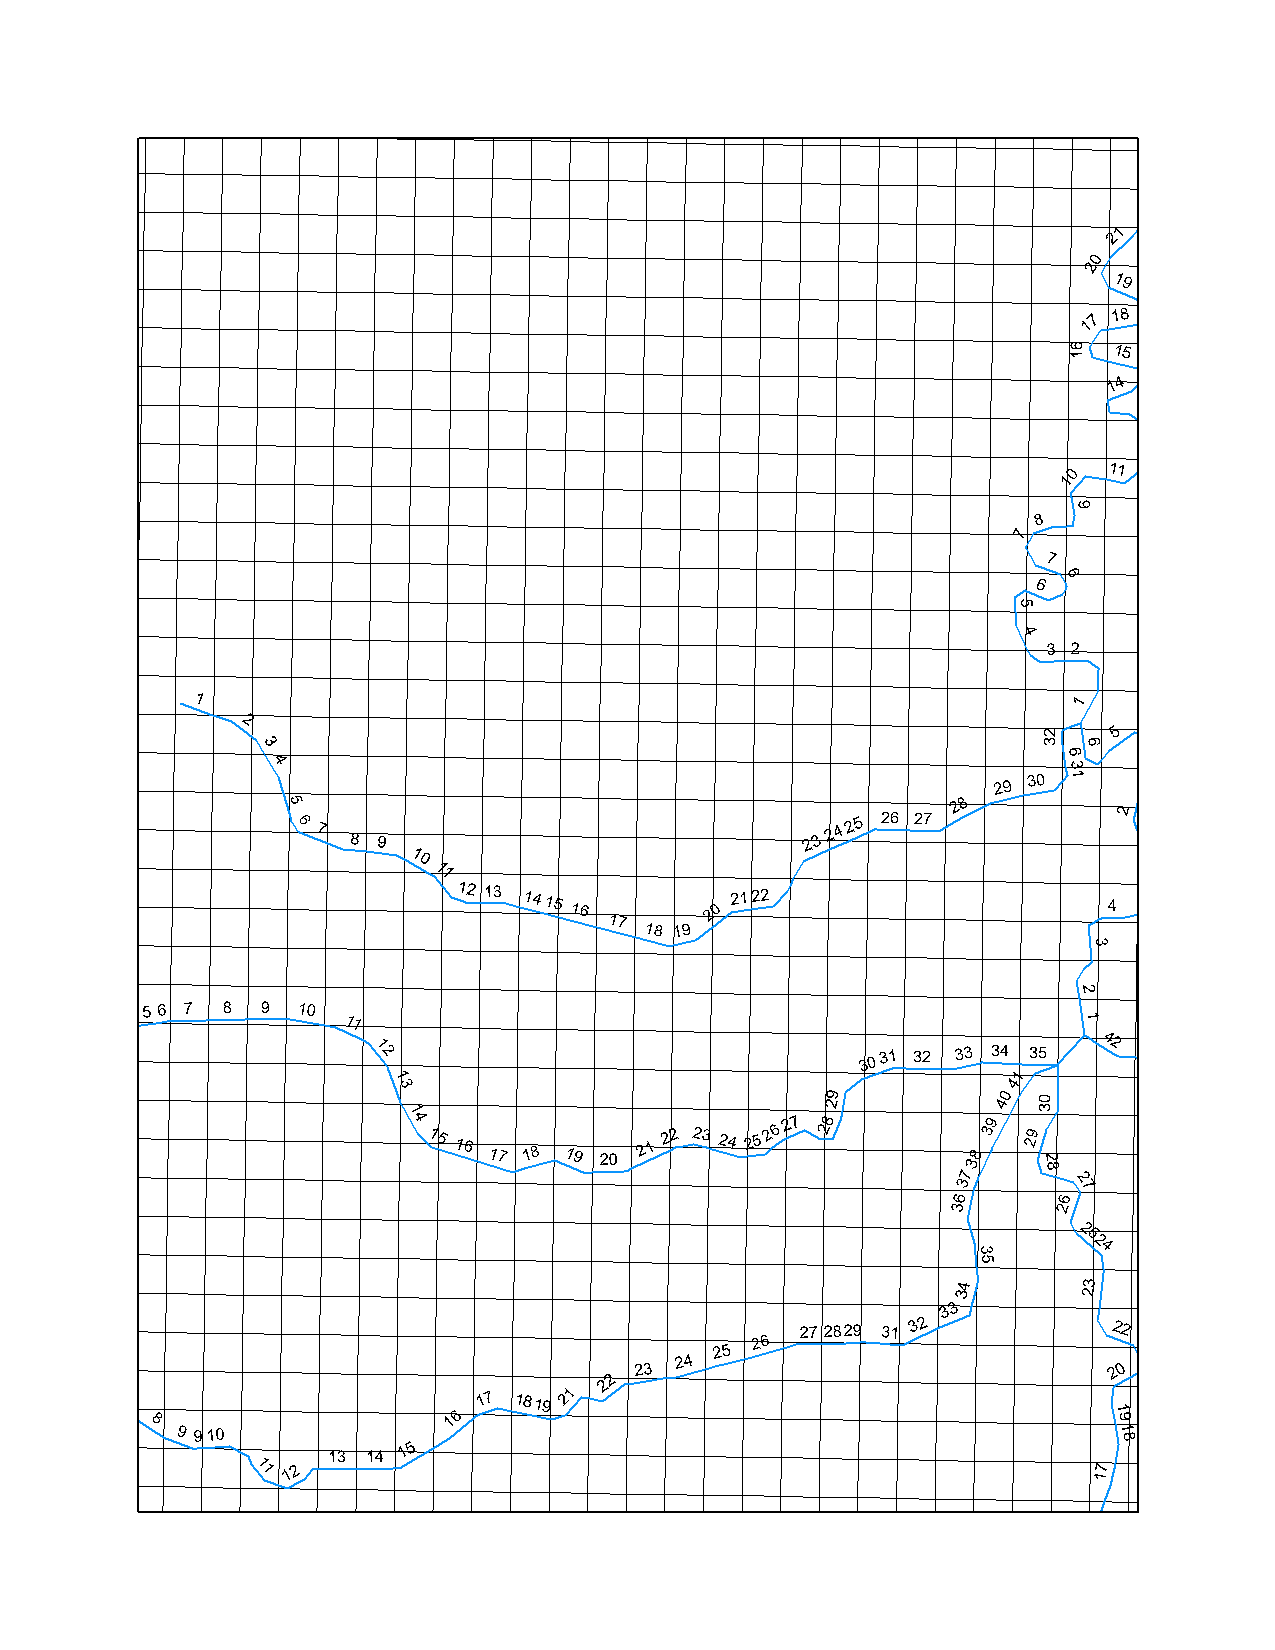
\includegraphics[scale=0.4]{reaches.png}
	\caption{Part of MODFLOW grid showing stream segments with reaches labelled.}
	\label{fig:reaches}
\end{figure}

The NHDPlus dataset includes `hydro-smoothed' elevations for each COMID, these elevations are 
generated during the processing of the NHDPlus to ensure that the network is routed downstream. The
python scripts written to process NHDPlus use the maximum and minimum smoothed elevations and 
interpolate linearly along the segment to assign an elevation of the streambed for each MODFLOW
grid cell.  The initial estimate for streambed elevation for each cell gives a routed system, although
this network has to be modified to account for streams that leave a cell, meander through one or
more cells, and then re-enter the original cell.  The elevation assigned to all the cells in the
meander has to be the same to avoid backwater conditions in the meander.

\begin{figure}[ht]
	\centering	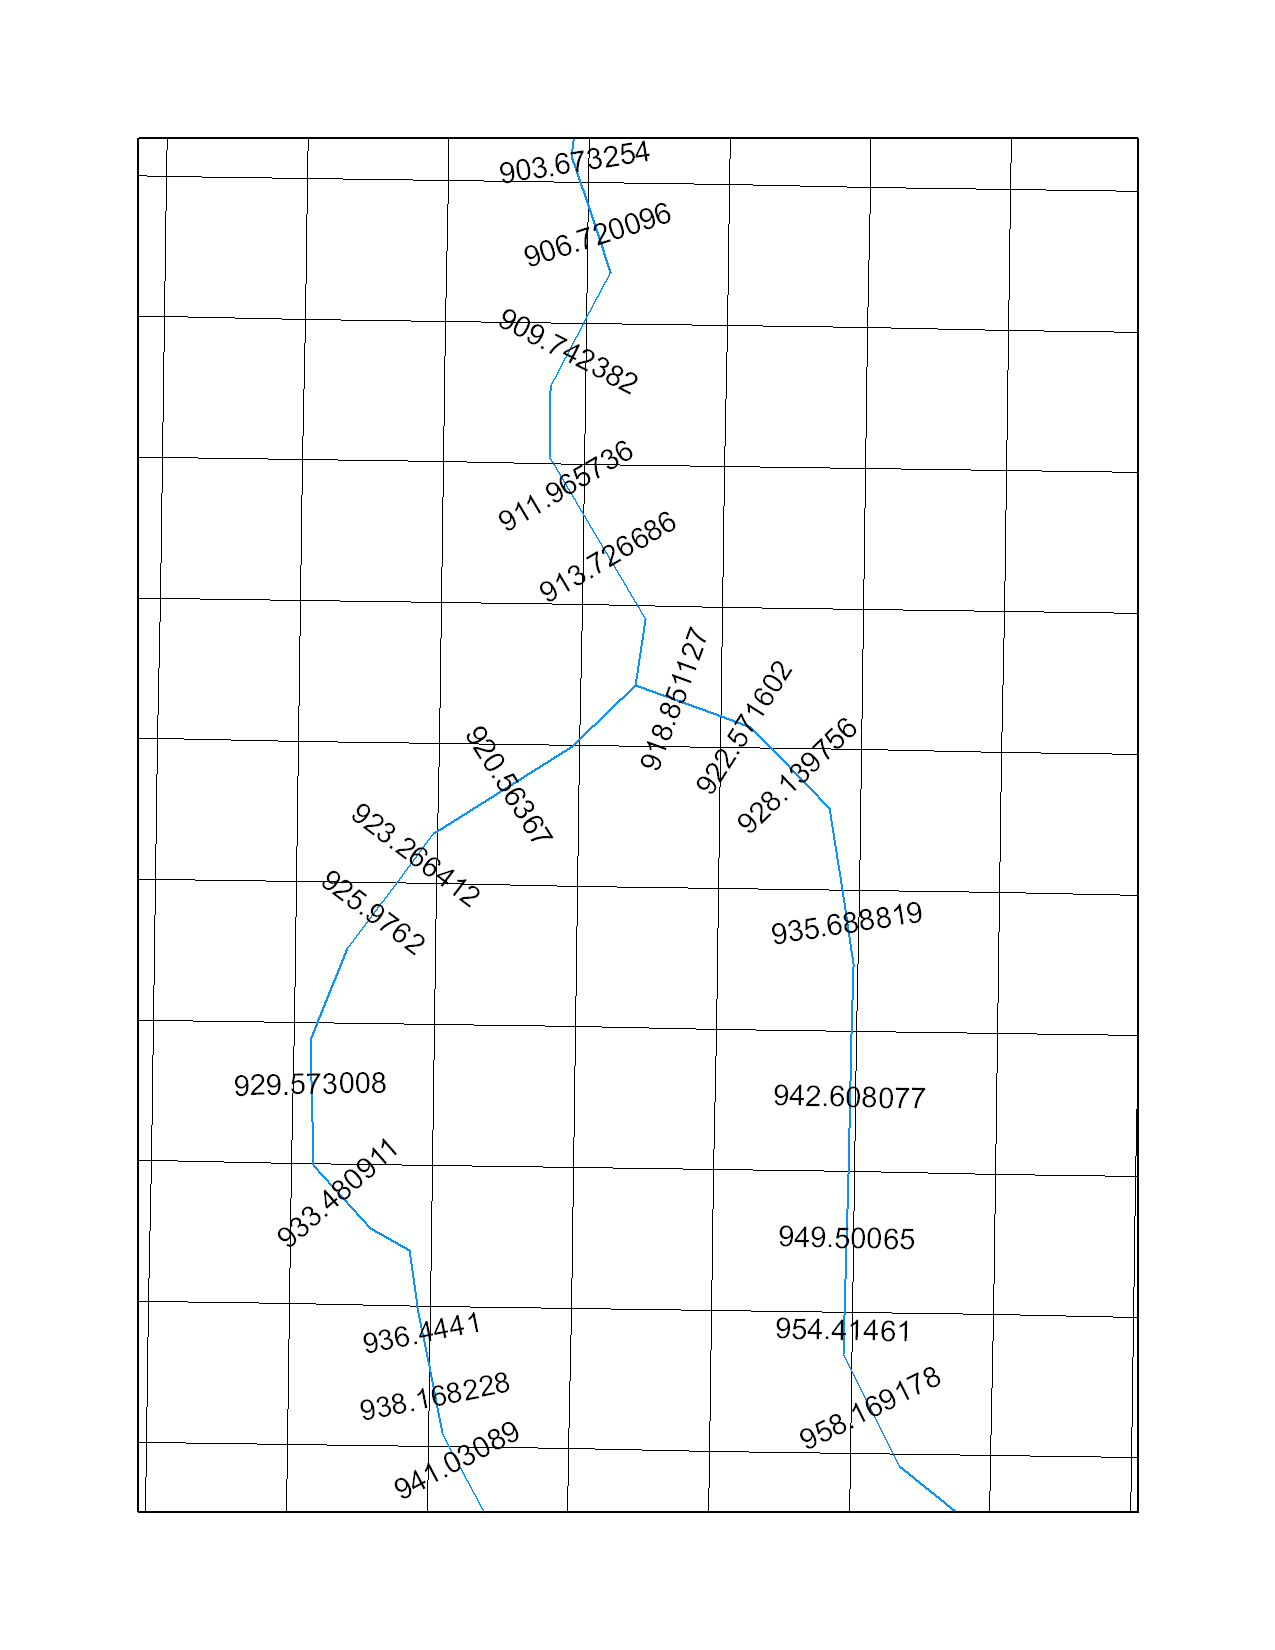
\includegraphics[scale=0.4]{elevations.png}
	\caption{Part of MODFLOW grid with stream reaches labelled with streambed elevation.}
	\label{fig:elevations}
\end{figure}

The biggest challenges to the current scripts are (1) mismatch between the elevation assigned to the
grid cell and the minimum or maximum smoothed elevation at the segment ends, and (2) streambed elevations
that are assigned to be above the elevation of the top MODFLOW grid cells, that is the land surface, (floating reaches) or too far below 
the land surface (incised reaches). The first condition happens where there is a mismatch
between the elevations assigned to the MODFLOW grid and the smoothed elevations in NHDPlus.
Either condition can happen
even if the ends of the segments are consistent with the MODFLOW grid if the change in the land
surface is significantly different than linear along the length of the stream.  Optimization of the problem may help produce
reasonable output files for regional problems.

\section{Proposed Optimization}

We propose to develop a program to optimize the streambed elevations of the network by solving
the following constrained minimization problem:

\begin{eqnarray}
 \min(F({\mathbf x}))  & =  & W_f (x-(G+\mathrm{float}))^p \  \mathrm{if} \ x > G+\mathrm{float} \label{eq:opt}\\
\  & = &  0 \ \mathrm{if} \  G+\mathrm{float} > x > G-\mathrm{incise} \nonumber \\
\  & = &  W_i ((G-\mathrm{incise})-x)^p \  \mathrm{if} \ x < G-\mathrm{incise} \nonumber 
\end{eqnarray}

\noindent where,
\begin{tabular*}{6.0in}[t]{lcl}
$F({\mathbf x})$ & = & function to minimize \\
${\mathbf x}$ & = & vector of streambed elevations \\
$W_f$ & = & weighting factor to penalize floating reaches  \\
$W_i$ & = & weighting factor to penalize extremely incised reaches  \\
float & = & acceptable amount a streambed can float above the grid cell \\
incise & = & acceptable amount a streambed can be incised below land surface \\
$x$ & = & streambed elevation in a MODFLOW grid cell \\
$G$ & = & land surface elevation \\
$p$ & = & power to raise residual \\
\end{tabular*}
\vspace{12pt}

\noindent Subject to the constraint,
\begin{equation}
	{\mathbf A}{\mathbf x} \geq 0  \label{eq:constraint}
\end{equation}

\noindent where ${\mathbf A}$ is a sparse matrix with the value $1$ designating the reach and
$-1$ designating the next downstream reach.  The inequality 
enforces that the change in elevation from the upstream reach to the next downstream reach has to be
greater than zero.

There also may be cells with fixed streambed elevations, for example the first segments of headwater streams
that are already consistent with the land surface elevation, 
\begin{equation}
	{\mathbf B} {\mathbf x} = {\mathbf b}  \label{eq:fixed}
\end{equation}

\noindent The fixed elevations can either be handled as a constraint of the problem or explicitly removed from the minimization problem.

There is a great deal of literature and available software packages to solve this type of optimization
problem where method does not rely on derivatives of the function.  Finding a solution that 
minimizes floating and incision while enforcing that the network remained routed should be feasible and
would be a great advance in preparation of MODFLOW input files.  Because this level of sophisication is
not needed by most MODFLOW users outside of USGS, this type of processing in available pre-processors
seems unlikely.

Python code has been written to compute $F({\mathbf x})$ and ${\mathbf A}$ given reaches and segments that have been generated by existing scripts to develop the SFR input.

\newpage
\appendix{Python script to compute $F({\mathbf x})$ and ${\mathbf A}$}
\lstinputlisting{optimizeSFR.py}

\end{document}
